\section{Ejercicio 9}

El objetivo en esta sección es romper el algoritmo de probabilidades fijas pero no el de dinámicas. Presentamos el siguiente lote:

\begin{lstlisting}
# Tareas cortas y frecuentes
&A7,6,1
# Tareas largas y poco frecuentes
&B3,13,4
\end{lstlisting}

Intuitivamente, la idea es crear procesos que sean más o menos largos, y que tengan un período largo (para que tengan una prioridad fija baja).
Luego, hay que crear muchos procesos cortos que le saquen tiempo a los procesos largos. En nuestro lote la familia A es de procesos cortos y la B de procesos largos.

Los procesos de la familia A, en el scheduler de prioridad fija, van a sacarle la cpu siempre a los de la B.
Sin embargo, el scheduler de prioridad dinámica ``se da cuenta'' cuando la deadline de los procesos de familia B se acerca, y los prioriza cuando eso pasa.

\begin{figure}[h]
 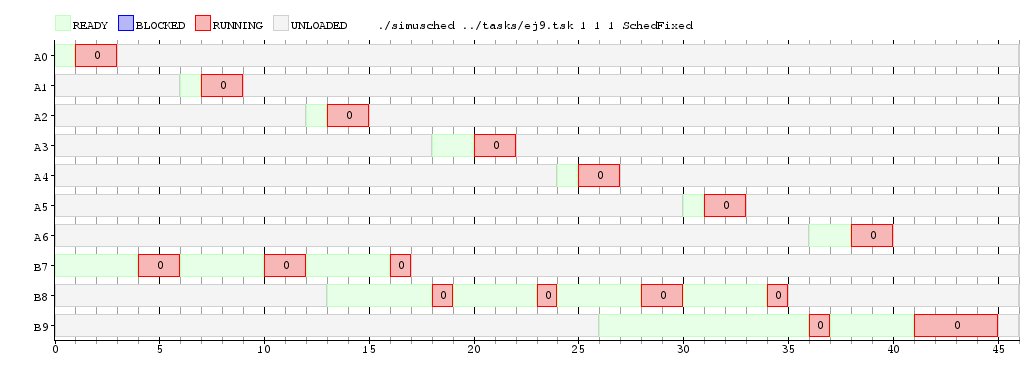
\includegraphics[width=\textwidth]{ej9/figs/fixed.png}
 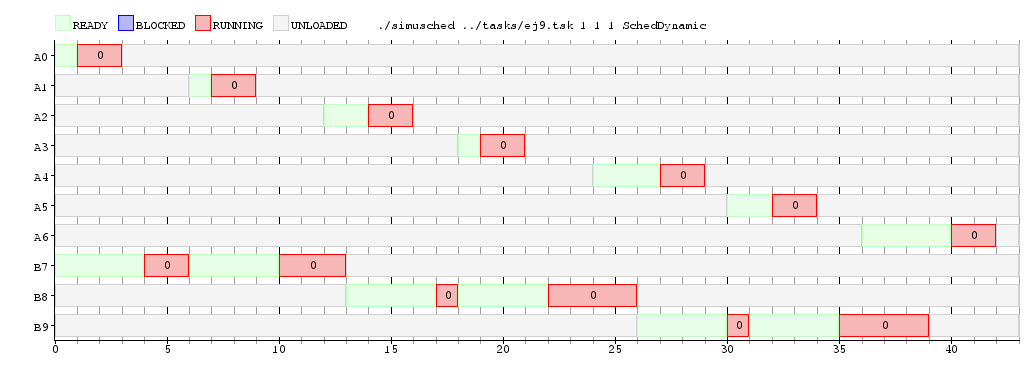
\includegraphics[width=\textwidth]{ej9/figs/dynamic.png}
 \caption{Diagramas de Gantt sobre el lote de tareas, para el algoritmo de prioridades fijas (arriba) y el de prioridades dinámicas (abajo).}
 \label{fig:ej9}
\end{figure}

Vemos en la figura~\ref{fig:ej9} que la deadline del proceso B7 no se cumple (tiene período 13 y se completa en el tick número 17).
En cambio en el algoritmo de prioridades dinámicas, se posterga la ejecución de A2 para poder cumplir la deadline de B7.
Esto no le impide terminar con el proceso A2 también.
